\oppgave{3}
Den største tilgjengelige verdien av bitenergi relativt til støytetthet er:
\[
    \left(\frac{E_b}{N_0}\right)_{\mathrm{dB}}=-0.450\enhet{dB}
\]
Den lineære verdien blir:
\[
    X=\frac{E_b}{N_0}=10^{-0.45/10}\approx0.902
\]
Vi betegner båndbreddeeffektiviteten med:
\[
    Y=\frac{C}{B}
\]
Bitenergien og støyeffekten kan uttrykkes som:
\[
    E_b=\frac{S}{C},\qquad N=N_0B
\]
Dette gir sammenhengen mellom signal-støyforhold og bitenergi:
\[
    \frac{S}{N}=\frac{E_bC}{N_0B}=XY
\]
Ved Shannon-grensen gjelder:
\[
    Y=\log_2\!\left(1+\frac{S}{N}\right)
\]
Vi setter inn uttrykket for signal-støyforholdet:
\[
    Y=\log_2(1+0.902Y)
\]
Her står den ukjente på begge sider. Vi løser derfor numerisk for den positive løsningen. Samme ligning kan skrives som:
\[
    \frac{2^Y-1}{Y}=0.902,\qquad Y>0
\]
For eksempel kan dette beregnes i Matlab/Octave uten ekstra toolbox:
\begin{verbatim}
X = 10^(-0.45/10);
f = @(Y) (2.^Y - 1)./Y - X;
Y = fzero(f, [0.7 0.75]);
C = 3100*Y;
disp(["Y = C/B =", num2str(Y)]);
\end{verbatim}
Den positive løsningen og største båndbreddeeffektiviteten blir:
\[
    \boxed{Y_{\max}\approx0.728\enhet{bps/Hz}}
\]
Løsningen $Y=0$ i den opprinnelige ligningen beskriver ingen informasjonsoverføring og er ikke den kapasiteten vi søker.

\newpage
Informasjonshastigheten innenfor den oppgitte båndbredden finnes fra:
\[
    C=Y_{\max}B
\]
Med $B=3100\enhet{Hz}$ blir dette, beregnet før avrunding av $Y_{\max}$:
\[
    C=Y_{\max}\cdot3100\approx2256.831\enhet{bps}
\]
Den teoretisk største informasjonshastigheten er dermed:
\[
    \boxed{C\approx2.257\enhet{kbps}}
\]
Som kontroll settes båndbreddeeffektiviteten tilbake i Shannon-uttrykket:
\[
    \log_2(1+0.902\cdot0.728)\approx0.728
\]
Figuren viser sammenhengen som brukes til å finne den positive løsningen:
\begin{figure}[H]
    \centering
    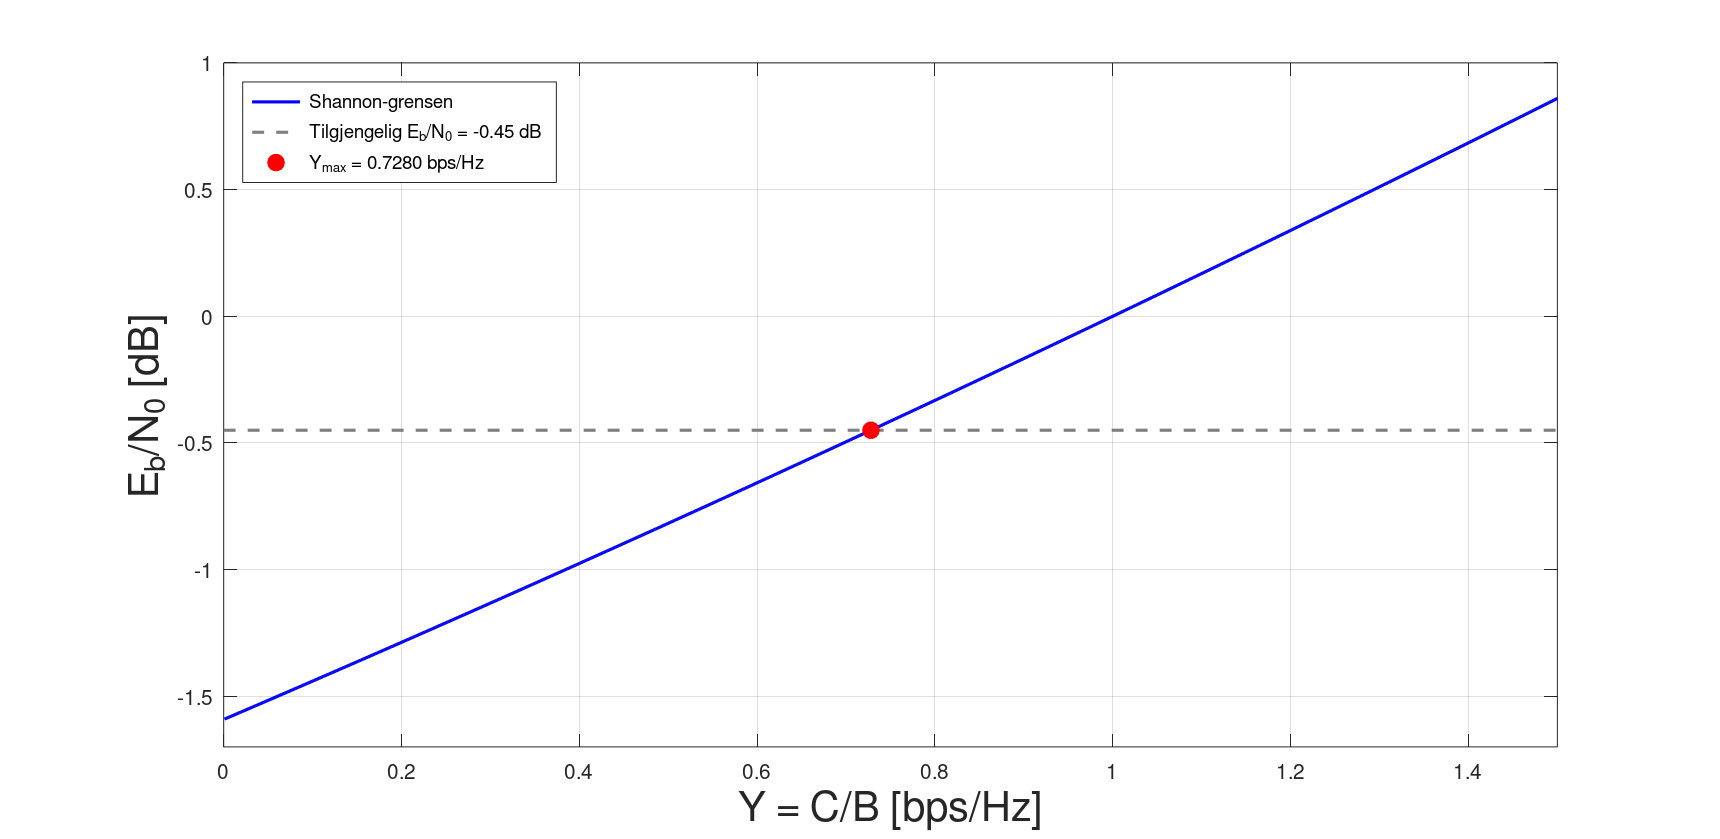
\includegraphics[width=\textwidth]{Media/grapf1.png}
    \caption{Shannon-grensen og tilgjengelig $E_b/N_0$ for undervannslenken.}
\end{figure}
